\providecommand{\main}{../../../..}
\documentclass[\main/dresen_thesis.tex]{subfiles}

\begin{document}
  \begin{figure}[!htbp]
    \centering
    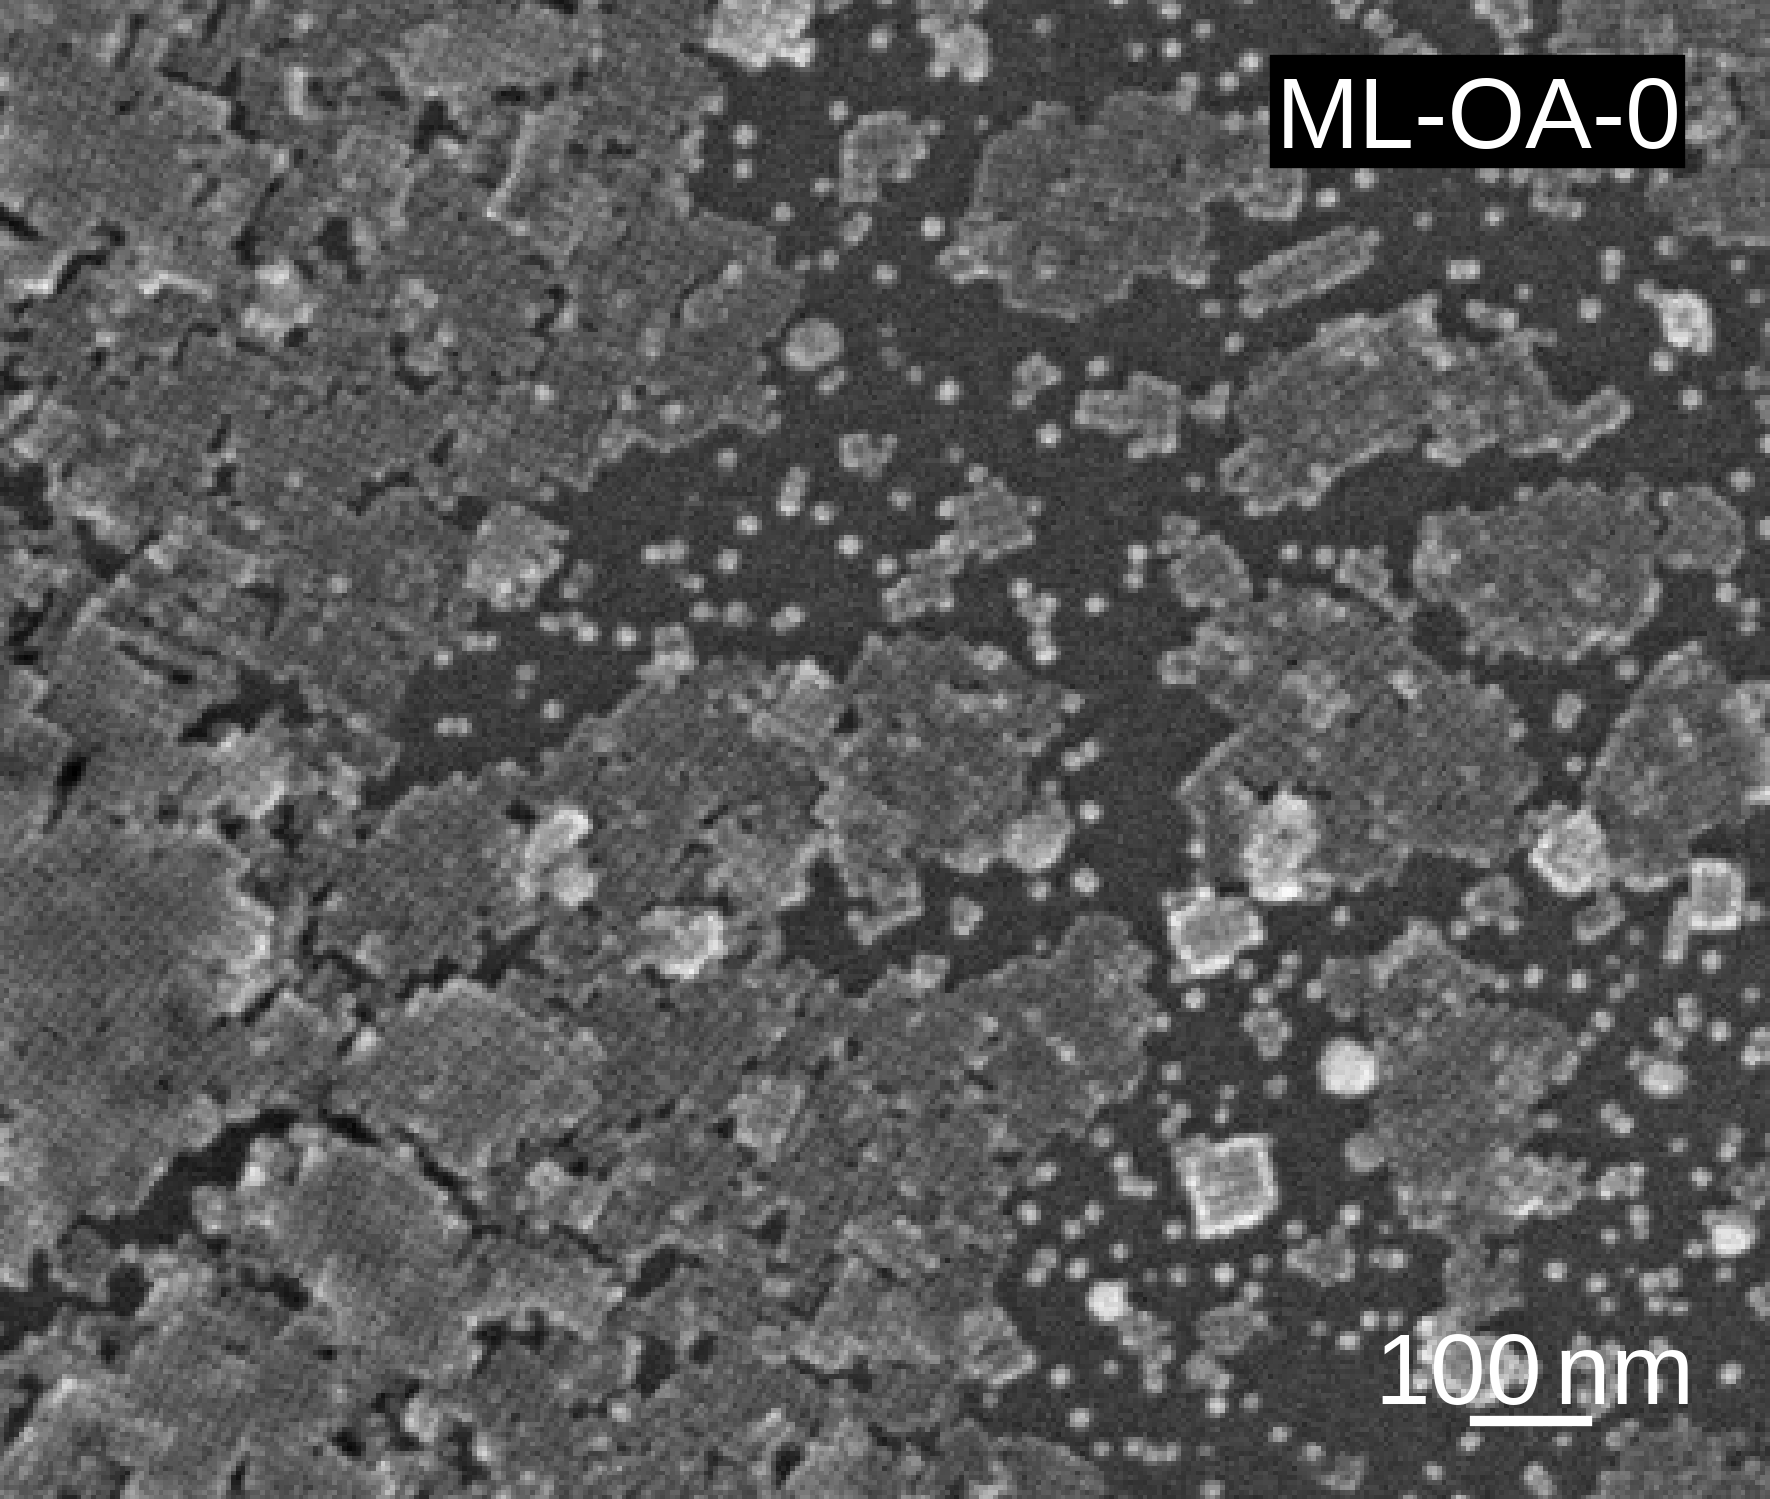
\includegraphics{monolayers_SEM_ML-OA-0}
    \caption{\label{fig:monolayers:preparation:solventVariation:NoOAAddend}SEM micrograph of Ac-CoFe-C-3 drop casted from a \textit{n}-heptane/octadecene dispersion.}
  \end{figure}

  % Additionally to the alkene additive that is added, the fraction of oleic acid in the dispersion plays a role in the self-assembly process.
  Excess oleic acid is naturally in the dispersion from the synthesis procedure as became visible in the SANS characterization of the dispersions in \refsec{sec:monolayers:nanoparticle:sas}.
  It is essential for the stabilization of the nanoparticles in dispersion, and a common trick to avoid precipitation of the nanoparticles, to add fresh oleic acid after redispersion \cite{Wetterskog_2014_Preci}.
  The exact volume fraction in a dispersion varies depending on the number of washing steps and which solvents are used during the purification process.
  From \reffig{fig:monolayers:preparation:solventVariation:NoOAAddend}, it is visible that drop casting Ac-CoFe-C-3 in the same combination of \textit{n}-heptane/octadecene as discussed in the previous section does not form a long range ordered array.
  Instead disconnected sheets of short-range ordered nanocubes are visible across the substrate and single nanocubes are sprinkled around them.
  As the oleic acid content in nanoparticle dispersions is not a strictly controlled parameter, the idea comes to mind that it's also important for the self-assembly process.

  To discuss which influence the oleic acid content has on the long range order formation, four dispersions from the same stock solution of Ac-CoFe-C-3 and only varied oleic acid content are shown in \reffig{fig:monolayers:preparation:solventVariation:OAAddend}.

  \begin{figure}[tb]
    \centering
    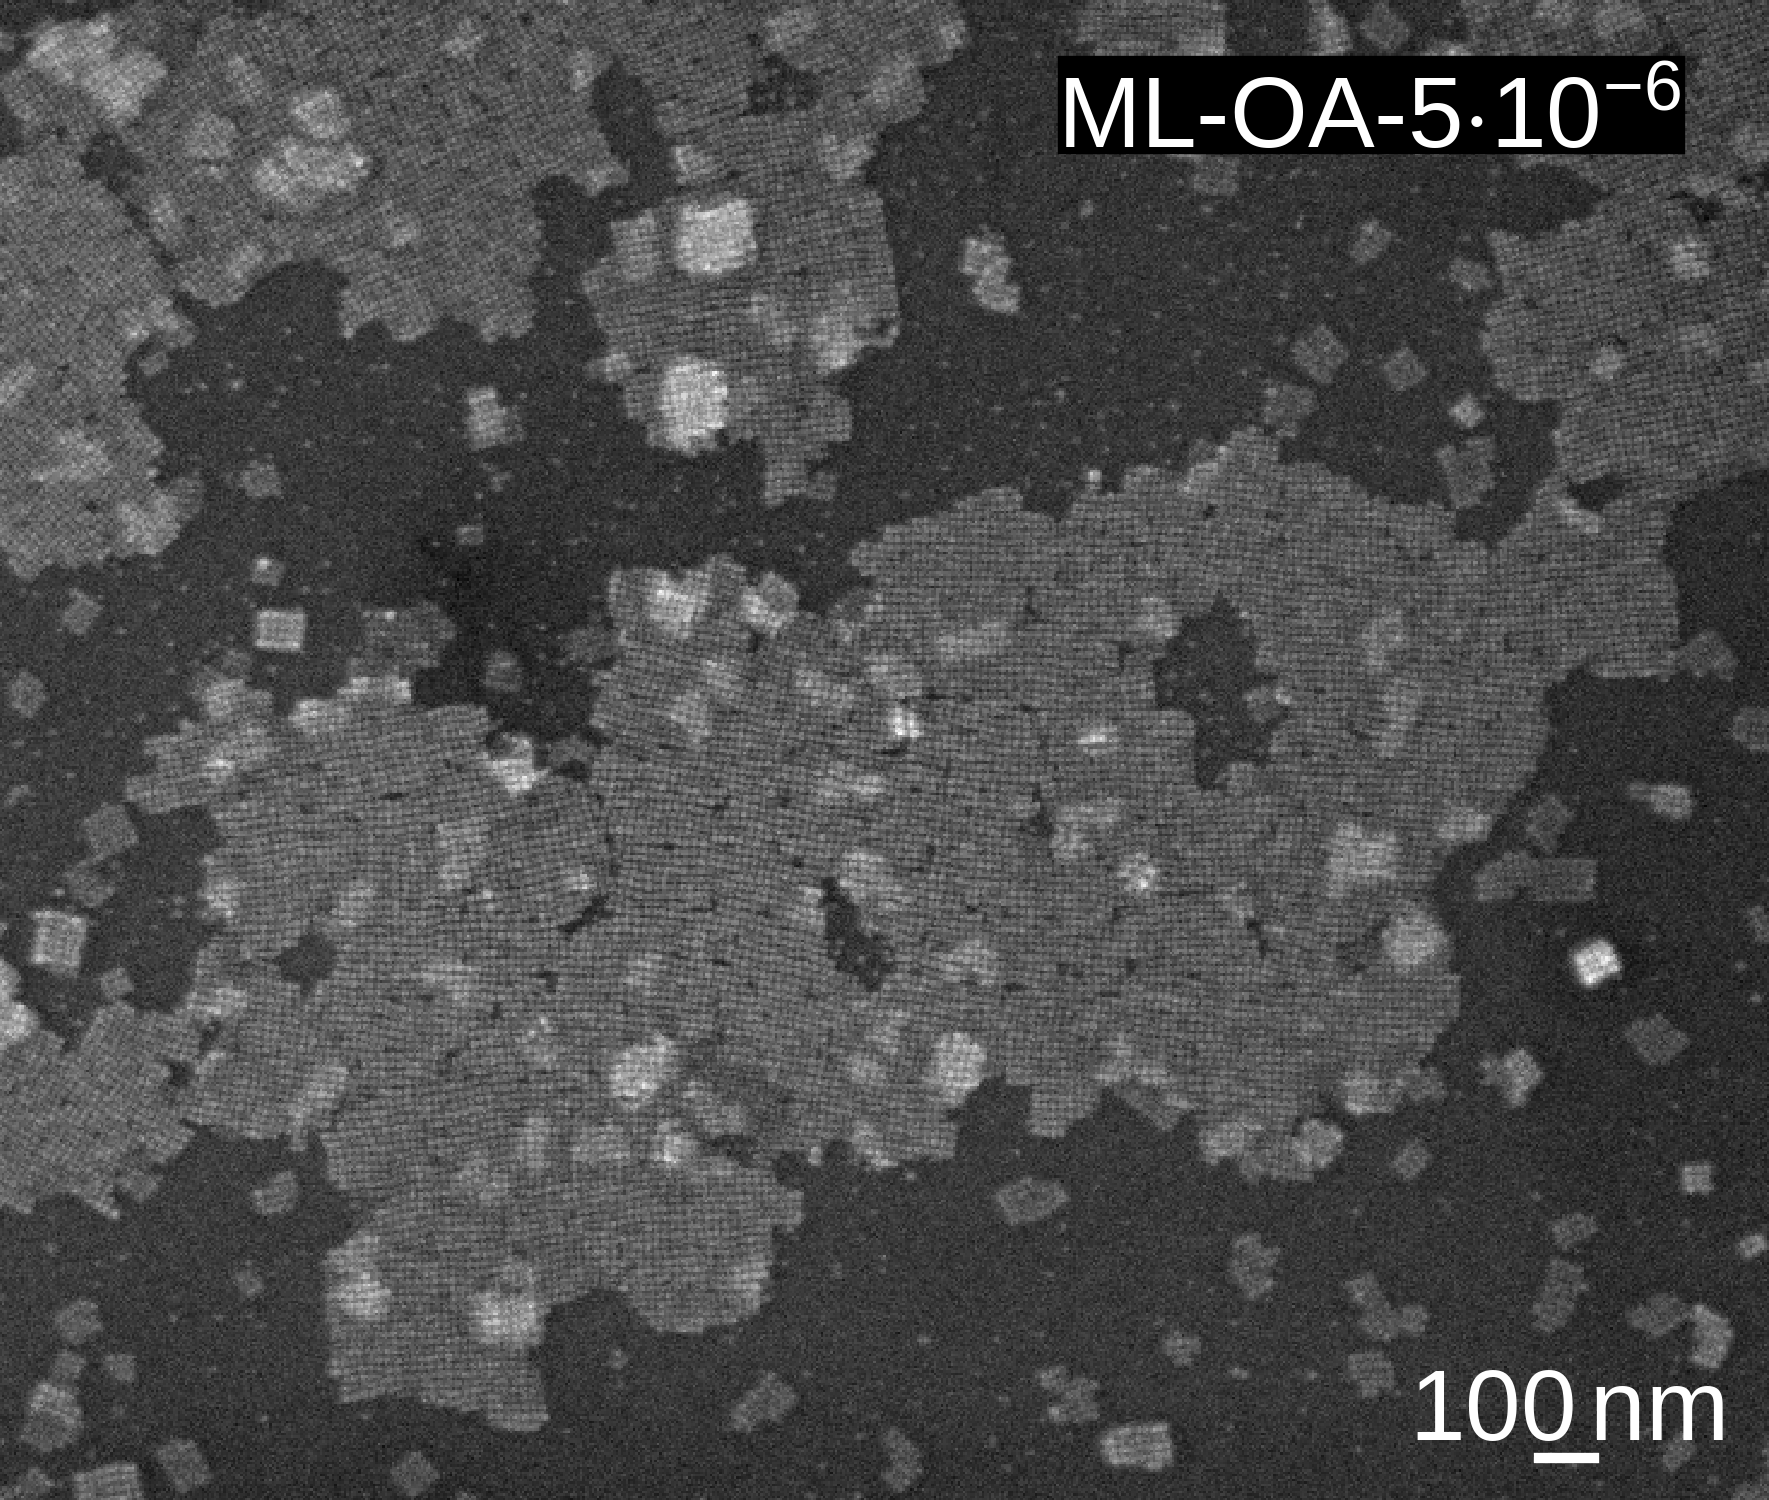
\includegraphics{monolayers_SEM_ML-OA-5e-6}
    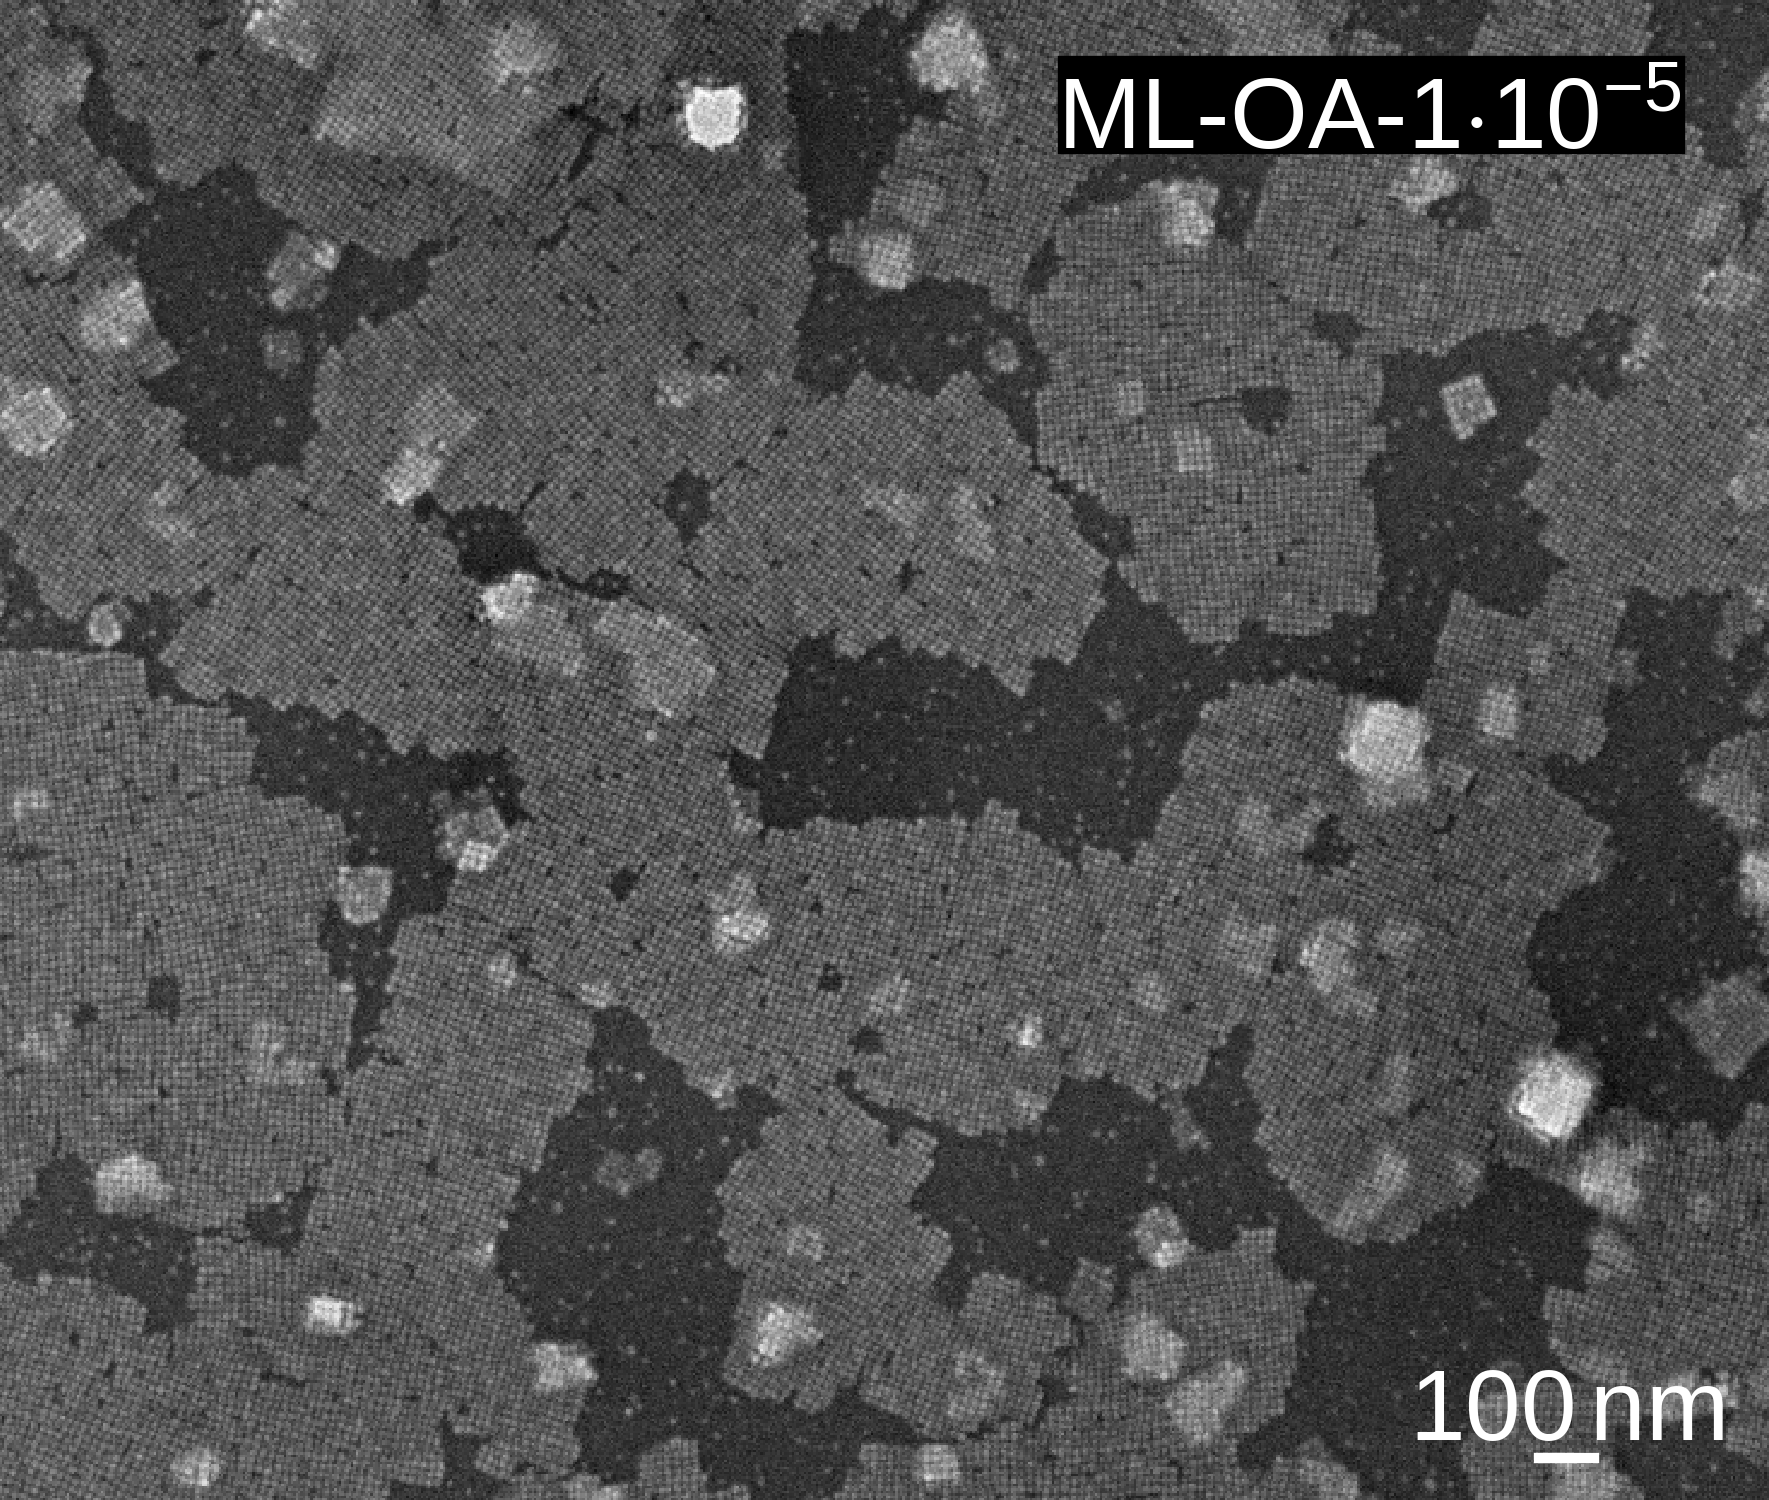
\includegraphics{monolayers_SEM_ML-OA-1e-5}
    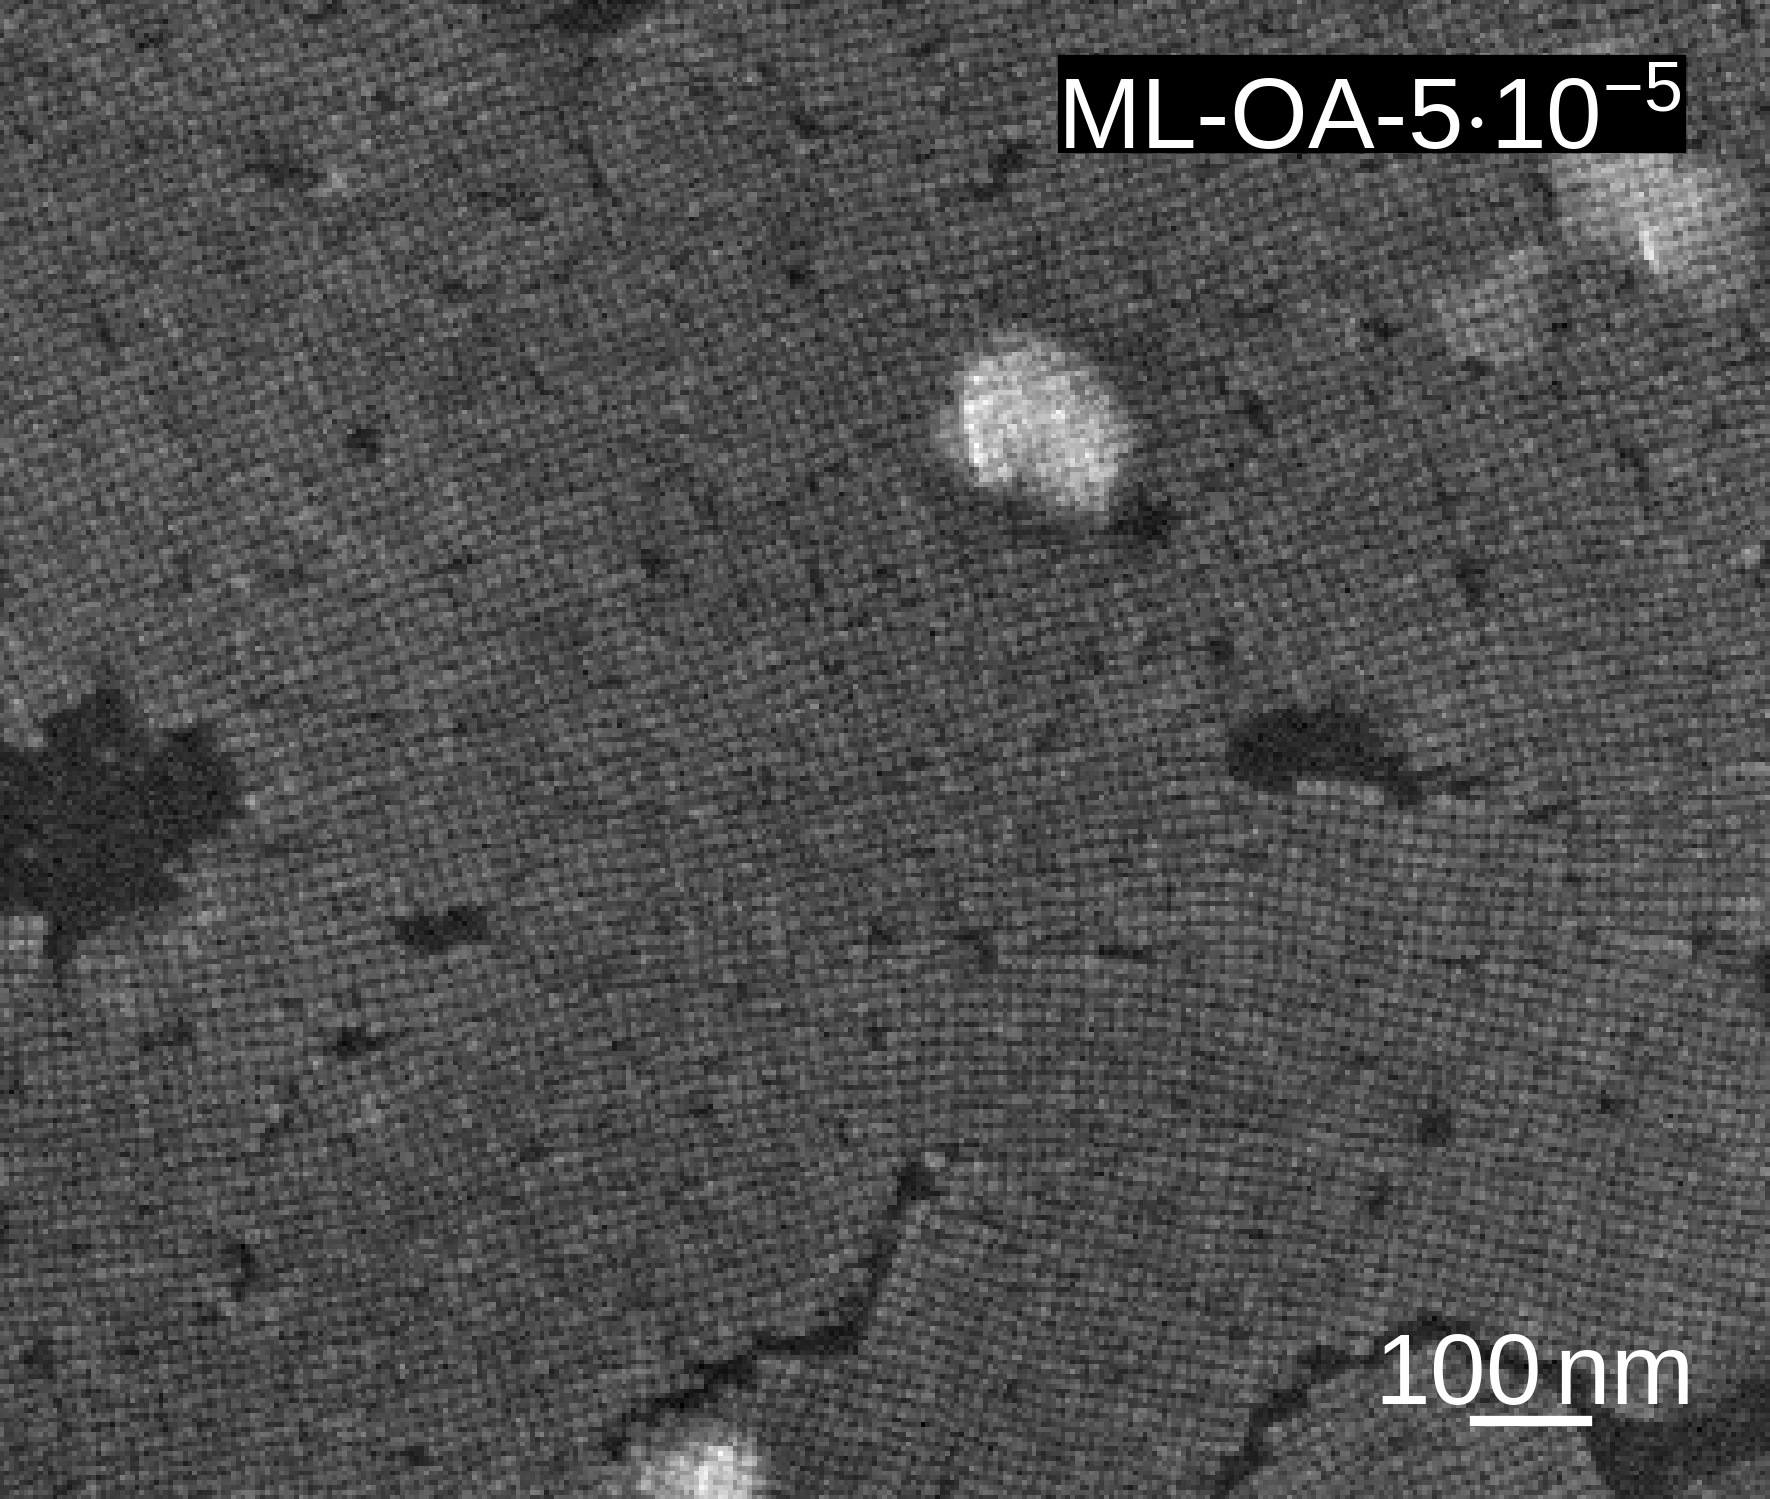
\includegraphics{monolayers_SEM_ML-OA-5e-5}
    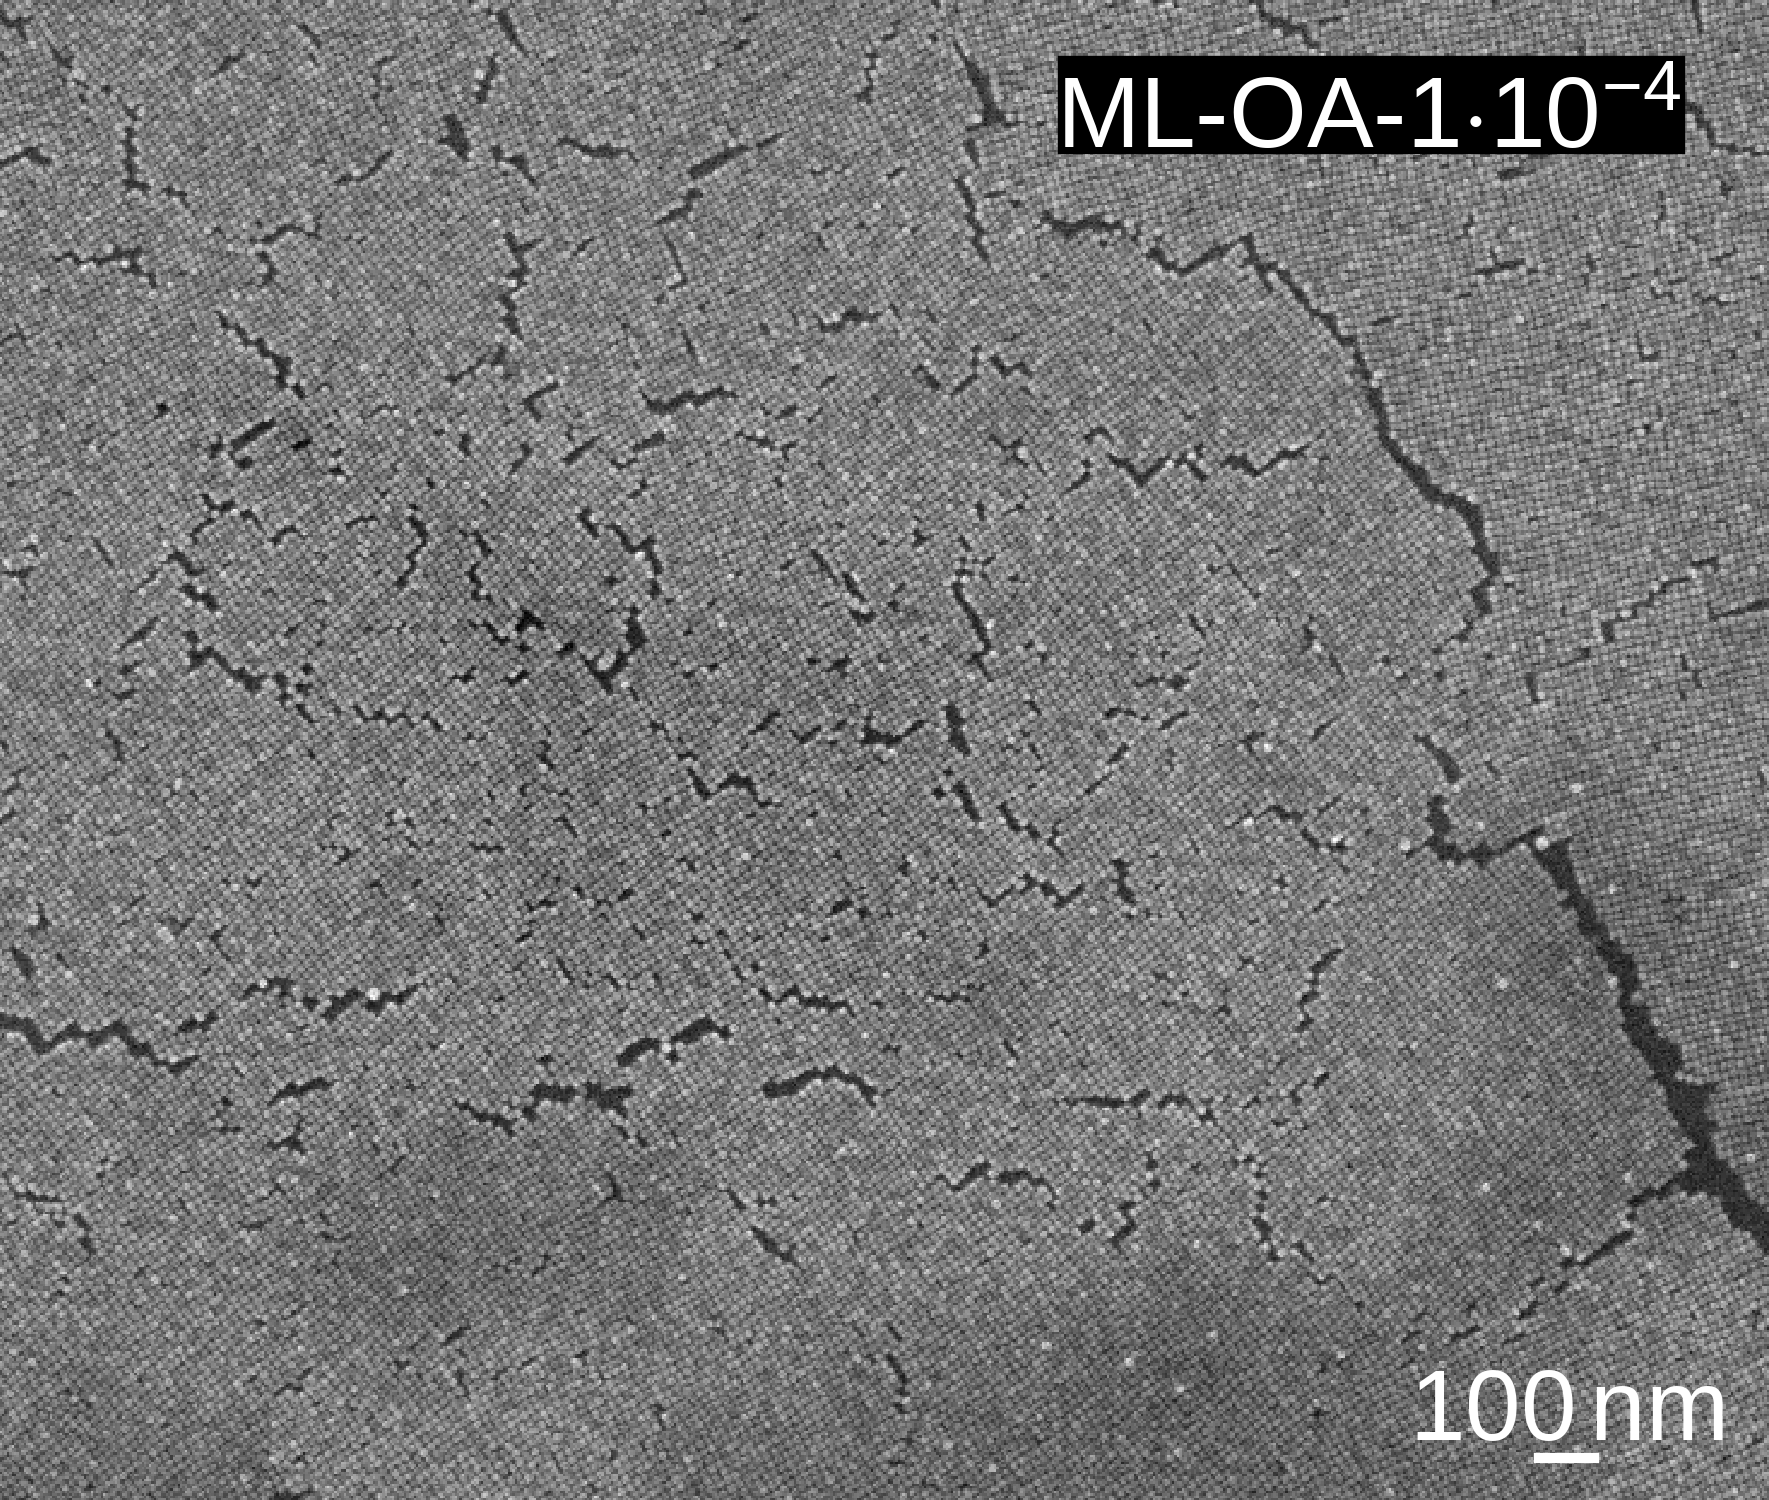
\includegraphics{monolayers_SEM_ML-OA-1e-4}
    \caption{\label{fig:monolayers:preparation:solventVariation:OAAddend}Variation of the oleic acid content analyzed in scanning electron microscopy. Monolayers drop casted from a dispersion of Ac-CoFe-C-3 with $5\cdot10^{-4} \unit{\%}$ (upper left), $1\cdot10^{-3} \unit{\%}$ (upper right), $5\cdot10^{-3} \unit{\%}$ (lower left) and $1\cdot10^{-2} \unit{\%}$ (lower right) oleic acid additive are shown.}
  \end{figure}

  The micrographs clearly show the trend for increasing long-ranged order with increase of the oleic acid content above $c_V^\textsf{OA} \eq 5\cdot10^{-3} \unit{\%}$.
  This concentration corresponds to a oleic acid film thickness of approximately $25 \unit{nm}$ if distributed homogeneously on the substrate surface.
  This coincides close to the nanocube size of approximately $12.5 \unit{nm}$.
  The amount of oleic acid that can be added to the dispersion is limited, as oleic acid is a solvent with a high boiling point ($T_\mathrm{bp} \eq 360 \unit{^\circ C}$) that is even more difficult to remove as 1-octadecene from a wafer after the drying of the primary solvent.
  It is reasonable to assume that the additional oleic acid during the final drying stage functions as a thin mobilization layer on which the nanocubes can still move in two dimensions, rearrange and reduce the defects in the lattice.
\end{document}